% chktex-file 1
% chktex-file 44
% chktex-file 45
% chktex-file 36
% chktex-file 3
% chktex-file 8
% chktex-file 18
% chktex-file 12
% chktex-file 13

\documentclass[twoside]{article}

\setlength{\headheight}{14.5pt}

\usepackage{graphicx,fancyhdr,amsmath,amssymb,amsthm,subfig,url,hyperref}
\usepackage{tikz}
\tikzset{main/.style={draw, circle, thick, minimum size=8mm}}

\usepackage[margin=1in]{geometry}
\newtheorem{theorem}{Theorem}


%---------------- IMPORTANT: Student and Homework Information -------------

%%% PLEASE FILL THIS OUT WITH YOUR INFORMATION
\newcommand{\myname}{Muhammad Mujtaba}
\newcommand{\myid}{28100480}
\newcommand{\hwNo}{Assignment 8}
%%% END



\fancypagestyle{plain}{}
\pagestyle{fancy}
\fancyhf{}
\fancyhead[RO,LE]{\sffamily\bfseries\large LUMS}
\fancyhead[LO,RE]{\sffamily\bfseries\large CS 210 Discrete Mathematics}
\fancyfoot[LO,RE]{\sffamily\bfseries\large \myname: \myid @lums.edu.pk}
\fancyfoot[RO,LE]{\sffamily\bfseries\thepage}
\renewcommand{\headrulewidth}{1pt}
\renewcommand{\footrulewidth}{1pt}

%--------------------- This is the title of the document. DO NOT CHANGE IT ------------------------

\title{CS 210 \hwNo}
\author{\myname \qquad Student ID: \myid}
\newcommand{\currentdate}{6 December 2025}
\date{\currentdate}

%--------------------------------- AFTER Entering the Student and Homework Information, write your answers below  ----------------------------------

\begin{document}
\maketitle

\section*{Question 1}

\begin{enumerate}
    \item[(a)] Linear, Homogenous (order 2) and Constant Coefficients exist
    \item[(b)] Linear, Order 1
    \item[(c)] Linear, Order 1, and Constant Coefficients exist
    \item[(d)] Not Linear or Homogenous, Order 2
    \item[(e)] Linear, Homogenous (order 3) and Constant Coefficients exist  
\end{enumerate}

\section*{Question 2}

\begin{enumerate}
    \item[(a)]  Interpretation of \(\binom{n-1}{k}\)  and \(\binom{n-1}{k-1}\) \\
                When choosing a team of size \(k\) from \(n\) scientists, fix a specific scientist, say \((X)\)
                \begin{enumerate}
                    \item[i.]  \(\binom{n-1}{k}\): Represents the number of ways to form the team excluding scientist \((X)\). All $k$ members are chosen from the remaining \(n-1\) scientists
                    \item[ii.] \(\binom{n-1}{k-1}\): Represents the number of ways to form the team including scientist \((X)\). Since \((X)\) takes one spot, we choose the remaining $k-1$ members from the remaining $n-1$ scientists
                \end{enumerate}
                Summing these gives Pascal's Identity: \(\binom{n}{k} = \binom{n-1}{k} + \binom{n-1}{k-1}\)
    \item[(b)]  To obtain $x^3 y^2$ from $(x+y)^5$, choose which 2 of the 5 factors contribute $y$.  
                The choices are \[\binom{5}{2} = 10\] 
    \item[(c)]  Using the Substitution Method (assume $n=2^k$):
                \[ T(n) = 2T\left(\frac{n}{2}\right) + 1 \]
                \[ = 2\left[2T\left(\frac{n}{4}\right) + 1\right] + 1 = 4T\left(\frac{n}{4}\right) + 2 + 1 \]
                \[ = 4\left[2T\left(\frac{n}{8}\right) + 1\right] + 2 + 1 = 8T\left(\frac{n}{8}\right) + 4 + 2 + 1\]
                \[ \vdots \]
                \[ = 2^k T\left(\frac{n}{2^k}\right) + \sum_{i=0}^{k-1} 2^i \]    
                At the base case $\frac{n}{2^k}=1$, so $T(1)=1$. The sum is a geometric series $2^k - 1$.
    
                \[ T(n) = n(1) + (n-1) \]
                \[ T(n) = 2n - 1 \]
\end{enumerate}


\newpage

\section*{Question 3}

\begin{enumerate}
    \item[(a)]  Impossible.  \\
                A vertex of degree $n-1$ is adjacent to all other vertices.  \\
                The vertex of degree 0 would be adjacent to it, contradiction. 
    \item[(b)]  Impossible.  \\
                A cubic graph on 5 vertices has total degree \(5 \cdot 3 = 15\), which must be even.  \\
                Contradiction.
    \item[(c)]  Impossible.  \\
                A bipartite graph on 5 vertices has at most \(2\cdot 3 = 6\) edges. \\  
                Cannot have 7.
\end{enumerate}

\section*{Question 4}

\begin{enumerate}
    \item[(a)] 
                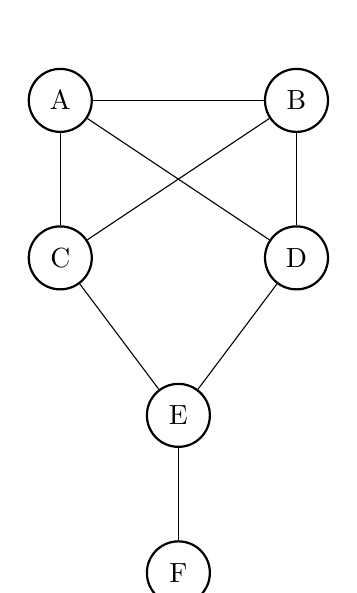
\begin{tikzpicture}[node distance= 2 cm]
                    \node[main] (A) at (0,4) {A};
                    \node[main] (B) at (3,4) {B};
                    \node[main] (C) at (0,2) {C};
                    \node[main] (D) at (3,2) {D};

                    \node[main] (E) at (1.5, 0) {E};
                    \node[main] (F) at (1.5, -2) {F};

                    \draw (A) -- (B);
                    \draw (A) -- (C);
                    \draw (A) -- (D);

                    \draw (B) -- (C);
                    \draw (B) -- (D);

                    \draw (C) -- (E);
                    
                    \draw (D) -- (E);

                    \draw (E) -- (F);
 
                 \end{tikzpicture}

    \item[(b)]
        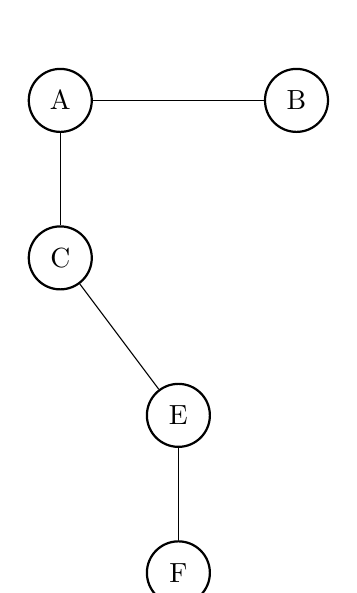
\begin{tikzpicture}[node distance=2cm]
            \node[main] (A) at (0,4) {A};
            \node[main] (B) at (3,4) {B};
            \node[main] (C) at (0,2) {C};
            \node[main] (E) at (1.5, 0) {E};
            \node[main] (F) at (1.5, -2) {F};

            \draw (B) -- (A); 
            \draw (A) -- (C); 
            \draw (C) -- (E); 
            \draw (E) -- (F); 
        \end{tikzpicture}

    \item[(c)]  Walk from A to F: \\
                Walk: \(A \to C \to E \to F\) \\
                Is it a path? Yes, because no vertices are repeated.

    \item[(d)]  Cycles in G:
                Yes. Example: \(A - B - C - A\) forms a triangle ($C_3$).

    \item[(e)]  Complement \(\overline{G}\): \\
                Edges in \(\overline{G}\): \((A,E), (A,F), (B,E), (B,F), (C,D), (C,F), (D,F)\) \\
                Connected? Yes. $F$ is connected to $A, B, C, D$. $E$ is connected to $A, B$ (which connect to $F$). All vertices are reachable. 
\end{enumerate}

\section*{Question 5}

\[  
    M = 
    \begin{bmatrix}
        0 & 1 & 1 & 0 & 0 \\
        0 & 0 & 1 & 1 & 0 \\
        0 & 0 & 0 & 1 & 0 \\
        0 & 0 & 0 & 0 & 1 \\
        1 & 0 & 0 & 0 & 0
    \end{bmatrix}
\]

\section*{Question 6}

\begin{enumerate}
    \item[(a)]  Minimum number of bridges for 6 islands to be fully reachable:  \[6 - 1 = 5.\]
                Any graph with fewer than $n-1$ edges is disconnected.

    \item[(b)]  Communication only allowed between nobles (4) and citizens (7): \\  
                Complete bipartite graph $K_{4,7}$ has  \[4 \times 7 = 28\] links.

    \item[(c)]  The network is bipartite: one part contains nobles, the other citizens, and all edges go between the two. \\  
                In a bipartite graph all cycles alternate between the two parts, so every cycle has even length. \\  
                Hence no odd cycle can exist.

\end{enumerate}

\end{document}
